\subsection{Glyph: \glyph{Not}}\label{sec:not}

The output of a \glyph{not} glyph is True if its input is False, and False otherwise.

\begin{glyphDescription}

\glyphSboTerm
SBO:0000238 ! not

\glyphIncoming One \glyph{logic arc} (\sect{logicArc}).

\glyphOutgoing

\glyphContainer
A \glyph{not} operator is represented by a circular shape containing the word ``NOT''.
The shape is linked to two ports, that are small arcs attached to the centres of opposite sides of the shape, as shown in \fig{not}.
The incoming \glyph{logic arc} (\sect{logicArc}) is linked to the extremity of the leftmost or uppermost port, while the outgoing \glyph{logic arc} (\sect{logicArc}) or \glyph{modulation} (\sect{modulation}) is linked to the extremity of the rightmost or bottommost port.

\glyphLabel
None.

\glyphAux
None.

\end{glyphDescription}

\begin{figure}[H]
  \centering
  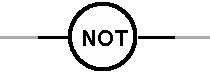
\includegraphics{images/build/not.pdf}
  \caption{The \PD glyph for \glyph{not}.}
  \label{fig:not}
\end{figure}
